\documentclass[12pt, a4paper]{report}

% Uncomment this to use Times New Roman (such as in IEEE, Elsevier)
\usepackage{mathptmx}

\title{A Web Application Firewall Using Reflex Agents}
\author{Abbhinav Bharadwaj}
\date{December 2025}

% Package imports
\usepackage{graphicx}
\usepackage{wrapfig}
\usepackage[a4paper, 
left=1.5in,
right=1in,
top=1in,
bottom=1in
]{geometry}
\usepackage{setspace}
\usepackage{tocloft} % optional, but neat
\usepackage{titlesec}
\usepackage{tikz}
\usepackage{url}
\usepackage{listings}
\usepackage{microtype}
\usepackage{longtable}

% Package configurations (paths, constants)
\graphicspath{{images/}}
\usetikzlibrary{arrows.meta, positioning, shapes.geometric, calc}
\setlength{\parskip}{6pt}
\setlength{\parindent}{0pt}
\renewcommand{\bibname}{REFERENCES}

% Definitions
\titleformat{\chapter}
{\normalfont\bfseries\fontsize{15}{18}\selectfont\MakeUppercase}
{\thechapter}
{1em}
{}
\titleformat{\section}
{\normalfont\bfseries\fontsize{12}{14}\selectfont\MakeUppercase}
{\thesection}
{1em}
{}
\titleformat{\subsection}
{\normalfont\itshape\fontsize{12}{14}\selectfont}
{\thesubsection}
{1em}
{}


\begin{document}
% Optional front page
\maketitle
\pagenumbering{roman}
% Official front page 	
{\centering
\large{A} \\
\Large{Project Report} \\
\large{on} \\
\Large{\textbf{A Web Application Firewall Using Reflex Agents}} \\
\vspace{5pt}
\large{by} \\
\large{Abbhinav Bharadwaj (2300970100003)} \\
\large{Under the supervision of} \\
\large{Prof. Mukesh Kumar Singh}

\begin{figure}[h]
	\centering
	\includegraphics[width=0.25\textwidth]{logo}
\end{figure}
\Large{\textbf{Computer Science and Engineering}} \\
\vspace{5pt}
\Large{\textbf{Galgotia's College of Engineering \& Technology}} \\
\large{Greater Noida, Uttar Pradesh} \\
\large{India - 201306} \\
\large{Affiliated to}

\begin{figure}[h]
	\centering
	\includegraphics[width=0.25\textwidth]{aktu}
\end{figure}
\Large{\textbf{Dr. A.P.J. Abdul Kalam Technical University}}\\
\large{Lucknow, Uttar Pradesh, India-226031}\\
\large{December 2025}

}

\newpage

\noindent % Prevents indentation shifting the logo
\begin{minipage}{0.15\textwidth}
	% FIX: Added closing ']' and '}' below
\includegraphics[width=1.1\linewidth]{logo} 
\end{minipage}%
\hfill % Pushes the text block slightly to the right
\begin{minipage}{0.85\textwidth}
\centering
{\Large \textbf{GALGOTIA'S COLLEGE OF} 
\\
\textbf{ENGINEERING \& TECHNOLOGY}
} \\
\small{GREATER NOIDA, UTTAR PRADESH, INDIA - 201306}	
\end{minipage}

\vspace{0.5cm} % Adds space before the certificate text starts
\begin{center}
\large{\textbf{CERTIFICATE}}
\end{center}	
\vspace{0.5cm}

{
This is to certify that the project report titled \textbf{``A Web Application Firewall Using Reflex Agents''} submitted by \textbf{Mr. Abbhinav Bharadwaj [2300970100003]} to \allowbreak Galgotia's College of Engineering \& Technology, Greater Noida, Uttar Pradesh, affiliated to Dr. APJ Abdul Kalam Technical University Lucknow, U.P. in partial fulfillment for the award of Degree of Bachelor of Technology in Computer Science \& Engineering is a bonafide record of the project work carried out by them under my supervision during the year 2025-26. 
}

\vspace{2.5cm}

\noindent
\begin{minipage}[t]{0.45\textwidth}
	\textbf{Prof. Mukesh Kumar Singh} \\
	\textbf{Assistant Professor} \\
	\textbf{Dept. of CSE}
\end{minipage}%
\hfill
\begin{minipage}[t]{0.36\textwidth}
	\textbf{Dr. Pushpa Choudhary} \\
	\textbf{Professor and Head} \\
	\textbf{Dept. of CSE} 
\end{minipage}

\newpage

\noindent % Prevents indentation shifting the logo
\begin{minipage}{0.15\textwidth}
	% FIX: Added closing ']' and '}' below
\includegraphics[width=1.1\linewidth]{logo} 
\end{minipage}%
\hfill % Pushes the text block slightly to the right
\begin{minipage}{0.85\textwidth}
\centering
{\Large \textbf{GALGOTIA'S COLLEGE OF} 
	\\
	\textbf{ENGINEERING \& TECHNOLOGY}
} \\
\small{GREATER NOIDA, UTTAR PRADESH, INDIA - 201306}	
\end{minipage}

\vspace{0.5cm} % Adds space before the certificate text starts
\begin{center}
\large{\textbf{ACKNOWLEDGEMENT}}
\end{center}	
\vspace{0.5cm}

I have taken my best efforts in this project. However, it would not be possible without the kind support and help of many individuals and organizations. I extend my sincere thanks to all of them.

I am highly indebted to \textbf{Prof. Mukesh Kumar Singh} for his guidance and constant supervision. Also, I am highly thankful to them for providing necessary information and support in completing the project.

I am extremely indebted to \textbf{Dr. Pushpa Choudhary}, HOD, Department of Computer Science and Engineering, GCET and \textbf{Ms. Lopamudra Mohanty}, Mini Project Coordinator, Department of Computer Science and Engineering, GCET for their valuable suggestions and constant support throughout my project tenure.

I also express my sincere thanks to all faculty and staff members of Department of Computer Science and Engineering, GCET for their support in completing this project on time.

I also express gratitude towards my parents for their kind co-operation and encouragement which helped me in completion of this project. Our thanks and appreciations also go to our friends in developing the project and all the people who have willingly helped me out with their abilities.

\vspace{1cm}
\noindent\textbf{Abbhinav Bharadwaj} \\
\textbf{2300970100003}

\newpage

\begin{center}
\large{\textbf{ABSTRACT}}
\end{center}
\vspace{1cm}

\noindent
This project implements a Web Application Firewall by integrating reflex-agent–based decision making within a reverse proxy architecture. The system operates as middleware, inspecting incoming client requests and autonomously responding to potential threats in real time. Machine learning models are employed to monitor, detect, and act upon malicious patterns in HTTP payloads. Two common web vulnerabilities-SQL Injection[CWE-89] and Cross-Site Scripting (XSS)[CWE-79] are addressed using XGBoost and Support Vector Machine classifiers, respectively. Experimental evaluation demonstrates detection accuracies of 98.54\% for SQL Injection and 96.15\% for XSS, indicating the effectiveness of the proposed agentic framework in enhancing adaptive web application security.

\noindent\textbf{KEYWORDS:} \textit{Reflex Agents, Reverse Proxy, SQL Injection, XSS, Support Vector Machine, XGBoost} 

\newpage

\begin{center}
	\large{\textbf{CONTENTS}}
\end{center}

\noindent
\begin{tabbing}
	\hspace{14cm} \= \kill
	\textbf{Title} \> \textbf{Page} \\[0.5cm]
	
	CERTIFICATE \> ii \\
	ACKNOWLEDGEMENT \> iii \\
	ABSTRACT \> iv \\
	CONTENTS \> v \\
	LIST OF TABLES \> vi \\
	LIST OF FIGURES \> vii \\
	ABBREVIATIONS \> viii \\
\end{tabbing}

\vspace{0.5cm}

\noindent
\begin{tabbing}
	\hspace{14cm} \= \kill
\textbf{CHAPTER 1: INTRODUCTION} \> 1-4 \\ \\

\textbf{CHAPTER 2: LITERATURE REVIEW} \> 5-12 \\

\textbf{CHAPTER 3: PROBLEM FORMULATION} \> 13\\

\textbf{CHAPTER 4: PROPOSED WORK} \> 14 \\

\textbf{CHAPTER 5: SYSTEM DESIGN} \> 15-16 \\

\textbf{CHAPTER 6: IMPLEMENTATION} \> 17-18\\

\textbf{CHAPTER 7: RESULT ANALYSIS} \> 19 \\

\textbf{CONCLUSION, LIMITATION, AND FUTURE SCOPE} \> 20\\

\textbf{REFERENCES} \> 21-22\\

\end{tabbing}
\newpage
\begin{center}
	\textbf{LIST OF TABLES}
\end{center}
\begin{enumerate}
	\item Table 2.1: Results from survey on ML\&DL for SQLi by Habib (2024)[14] \dotfill 7
	\item Table 7.1: Results and analysis \dotfill 19
\end{enumerate}
\newpage
\begin{center}
	\textbf{LIST OF FIGURES}
\end{center}
\begin{enumerate}
	\item Figure 1.1: Workflow of a Web Application Firewall \dotfill 3
	\item Figure 1.2: OWASP Top 10 2021 Comparison from OWASP[6] \dotfill 4
	\item Figure 1.3: Top 5 from CWE Top 25, 2025 \dotfill 4
	\item Figure 2.1: Architecture of a Random Forest Classifier \dotfill 11
	\item Figure 2.2: Random Forest Illustration (reproduced from Janosh[17]) \dotfill 11
	\item Figure 2.3: Architecture of a Support Vector Machine (SVM) Classifier \dotfill 12
	\item Figure 5.1: Architecture of Agentic WAF using Reflex Agents \dotfill 15
\end{enumerate}
\newpage
\chapter*{Abbreviations}
\addcontentsline{toc}{chapter}{List of Abbreviations}

\begin{tabular}{p{4cm} p{10cm}}
	AI   & Artificial Intelligence \\
	AJAX & Asynchronous Javascript and XML \\
	API  & Application Programming Interface \\
	B2B & Business-to-Business \\
	BiLSTM & Bidirectional Long Short-Term Memory \\
	CCP & Coding Copilot (Coding Agent) \\
	CNN  & Convolutional Neural Network \\
	CRS & Core Rule Set \\
	CSS & Cascading Style Sheets \\
	CVSS & Common Vulnerability Scoring System \\
	CVE & Common Vulnerabilities and Exposures \\
	CWE & Common Weakness Enumeration \\
	CSP & Content Security Policy \\
	CSRF & Cross-Site Request Forgery \\
	DL & Deep Learning \\
	DOM & Document Object Model \\
	HTML & Hypertext Markup Langugae \\
	HTTP & Hypertext Transfer Protocol \\
	HTTPS & Hypertext Transfer Protocol Secure \\
	IT & Information Security \\
	LLM & Large Language Model \\
	ML   & Machine Learning \\
	OWASP & Open Worldwide Application Security Project \\
	PoLP & Principle of Least Privilege \\
	PDCGs & Prompt Driven Code Generators (Generative AI) \\
	PHP & Hypertext Preprocessor \\
	RF   & Random Forest \\
	SaaS & Software as a Service \\
	SQL  & Structured Query Language\\
	SQLi & SQL Injection \\
	SVM  & Support Vector Machine \\
	TF-IDF & Text Frequency - Inverse Document Frequency \\
	WAF  & Web Application Firewall \\
	XGBoost & eXtreme Gradient Boosting \\
	XML & Extensible Markup Language \\
	XSS  & Cross-Site Scripting \\
\end{tabular}


\newpage 
 \clearpage
 \pagenumbering{arabic}
\chapter{Introduction}
Web Application Security is among the fastest evolving domains in Computer Science. With the adaptation of new technologies built on top of each other, from PHP and AJAX with MySQL to Node and React with MongoDB, a thorough assessment of security reveals it did not decrease security risks, but made them complicated enough to be in the developer's oversight\cite{iannone2023secretlife}. With the rise of modern AI agents in modern application development, for developing parts with Prompt Driven Code Generators (PDCGs) and applications as a whole with Coding Copilots (CCPs) (often referred to as \textit{Vibe Coding}), it becomes important we reexamine how application security can be ensured\cite{Mohsin2024TrustingLLMCode}. Though Agents are on average better than human developers in writing secure code\cite{asare2023githubcopilot}, their training data and method of operation can lead to inconsistencies in security performance\cite{chang2023survey}. 

\section{Background}
Web Applications are centric to the modern digital landscape. With the surge in number of internet users, there is an increase in businesses preferring web based services over Desktop and Android Applications due to lesser development and maintainence cost. This correlates with an increase in website usage over app usage in recent years\cite{Amplitude2022TrendReport}. With web solutions being accessible from a variety of devices and technologies, comes the challenge of web vulnerabilities. 
\subsection{OWASP Top 10}
The \textit{Open Worldwide Application Security Project (OWASP)} is a leading cybersecurity organisation that handles several central security projects, including the \textit{OWASP Top 10\cite{OWASP:Top10:2021}}. OWASP Top 10 is a standard awareness document released every 5 years, representing a broad consensus of most critical security risks to web applications. OWASP also maintains the \textit{Core Rule Set (CRS)}, a set of generic detection rules for protection from a wide range of attacks including the OWASP Top 10. It can be used with \textit{ModSecurity}, an open source Web Application Firewall, or other supporting applications. 
\subsection{CWE}
Common Weakness Enumeration, abbreviated as CWE, is a community maintained list of software and hardware weaknesses, often referred by the industry as a reliable resource. The CWE also maintains an yearly list of \textit{Top 25 Most Dangerous Software Weaknesses\cite{CWE:2025Top25}}.
\subsection{CVE}
Common Vulnerabilities and Exposures (CVEs) is a community driven catalog of publicly disclosed vulnerabilities\cite{cve_org}. It is more specific than the CWE index, hosting nearly 3,00,000 CVE Records open source.
\subsection{CVSS}
The \textit{Common Vulnerability Scoring System (CVSS)} is an open framework that provides a standardized way to rate the severity of computer security vulnerabilities, on a scale from 0.0 to 10.0, with 10.0 being the most severe. It considers how a vulnerability may be exploited (called as an \textit{Attack Vector}), how easily it is to exploit (called as \textit{Attack Complexity}), privileges required to perform the attack, \textit{et. cetera.}

\section{Emerging Landscape}
Cybersecurity awareness and security conscious development in the industry has made several once prevalent vulnerabilities nearly extinct, such as \textit{Path Traversal, Open Redirection, XML External Entities, Insecure Direct Object References, et. cetera.} However, building and maintaining secure systems remains a non trivial tasks today, with several dangerous vulnerabilities such as SQL Injection, Cross Site Scripting \textit{XSS}, Cross Site Request Forgery \textit{CSRF} and Remote Code Execution \textit{RCE} among others surviving till date. 
\subsection{Increasing Application Complexity}  
Modern applications comprise of several systems working together, including multiple APIs, Microservices, Cache Systems, Distributed Servers, SaaS Services, \textit{et. cetera} to provide cutting edge functionality and compete in meeting user requirements. This leads to an increase in attack surface, or potential points of attack. 
\subsection{Increasing Dependencies}
Development teams often use open-source and proprietary dependencies to speed up their development and ship the product as fast as possible. When a security vulnerability is found in a library, it affects all the dependent applications\cite{kumar2024vuln_deps_oss}. 
\subsection{Rise of Coding Agents}
With Generative AI advancements, LLMs such as ChatGPT, Gemini, Claude and Coding Agents such as Cursor, Warp, Claude Code allow users to write code with the highest level of abstraction. Since the training data can not be guaranteed to be secure, specially in large amounts, they are prone to writing insecure code\cite{Mohsin2024TrustingLLMCode}. Since AI Systems are non-deterministic and prompt-dependent, application security becomes a trade of luck and attention\cite{promises_pitfalls_llm_feedback_2024}.

\section{Modern Approaches to Application Security}
Most if not all, of IT and Software firms are now Cybersecurity aware. Security is a core component of any modern software product. 
\subsection{Cybersecurity Departments}
Leading software and IT firms have dedicated Cybersecurity departments, that are responsible for secure operations and actively handling security crises. 
\subsection{Security Aware Development Teams}
Developers are now security aware, and learn to follow safe code practices as a non-trivial part of their career. There exist journals for information regarding the trends in security to keep developers up to date. 
\subsection{Crowdsourcing}
There are Hacker communities that proactively discover vulnerabilities in applications, and report them for merit and monetary compensations. They are often referred to as \textit{White Hat Hackers} or \textit{Bug Bounty Hunters}. 
\subsection{Security Outsourcing}
Many firms outsource some or all of their security components, either to product based services such as a \textbf{Web Application Firewall} or to B2B SaaS products, such as Cloudflare, Orca, CrowdStrike, \textit{et. cetera.}

\section{Web Application Firewalls}
A traditional Web Application Firewall is a reverse proxy that intercepts incoming traffic to validate and sanitize or block the user request. Most of the application vulnerabilities can be catered by this approach.
\begin{figure}[h]
	\centering
	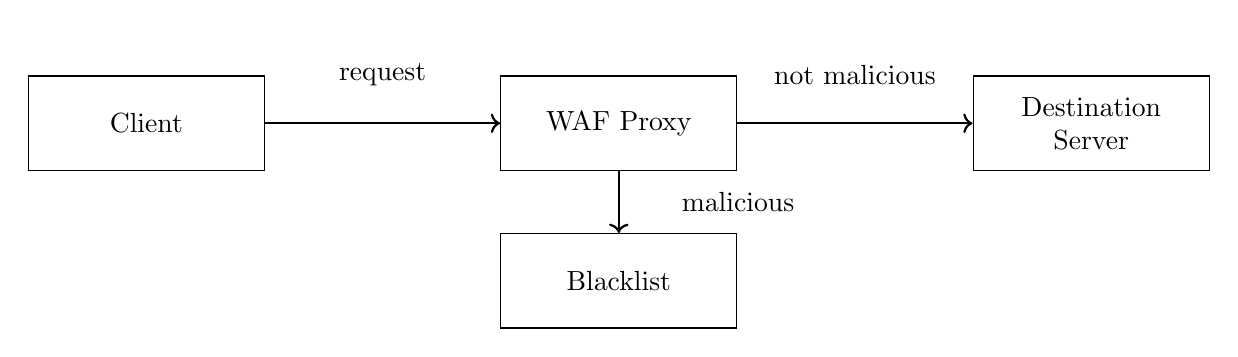
\begin{tikzpicture}[
		node distance=6cm,
		every node/.style={draw, rectangle, minimum width=3cm, minimum height=1.2cm, align=center},
		arrow/.style={->, thick}
		]
		
		% Nodes
		\node (client) {Client};
		\node (waf) [right of=client] {WAF Proxy};
		\node (server) [right of=waf] {Destination\\Server};
		\node (blacklist) [below of=waf, node distance=2cm] {Blacklist};
		
		% Arrows
		\draw[arrow] (client) -- node[above, draw=none]{request} (waf);
		\draw[arrow] (waf) -- node[above, draw=none]{not malicious} (server);
		\draw[arrow] (waf) -- node[right, draw=none]{malicious} (blacklist);
		
	\end{tikzpicture}
	\caption{Workflow of a Web Application Firewall}
\end{figure}
\subsection{Signature Based WAFs}
They use specific pre-defined attack patterns to block known threats. Incoming traffic is matched against a vast set of known signatures. 
\subsection{Rule Based WAFs}
They put reliance on strict rule sets, such as automatons or regular expressions to detect malicious user requests. One of the reputed rule sets is the OWASP CRS (Core Rule Set). The \textbf{Azure Web Application Firewall} incorporates the OWASP CRS. 
\subsection{WAF Agents} 
A part of active research, where the WAF has the ability to predict, act and adapt to cater to application security tasks. 

\section{Web Vulnerabilities}
\begin{figure}[h]
	\includegraphics[width=\linewidth]{owaspmapping}
	\caption{OWASP Top 10 2021 Comparison from OWASP\cite{OWASP:Top10:2021}}
\end{figure}
Figure 1.2 shows the change of trends in vulnerabilities from 2017 to 2021, where several vulnerabilities changed positions, and three rose to the Top 10 list. 
It is noted that XSS and SQL Injection, the primary targets of this project, are listed at ~$3^{rd}$~ rank. 

\begin{figure}[h]
	\includegraphics[width=\linewidth]{CWE2025}	
	\caption{Top 5 from CWE Top 25, 2025}
\end{figure}

CWE Top 25, 2025 as shown in figure 1.3, lists XSS at ~$1^{st}$~ rank and SQL Injection at ~$2^{nd}$~ rank. This highlights the importance and severity of the \textit{age-old } attack vectors in the modern landscape. Hence, We approach these vulnerabilities first in this project.  

\chapter{Literature Review}
\section{Introduction}
SQL Injections and XSS are severe vulnerabilities, and pose a major threat to any organization. Several approaches have been taken to mitigate the two attack vectors, by several direct and indirect means. 
\subsection{The state of SQL Injections}
A survey done by \textbf{Aikido}\cite{aikido_state_of_sql_injection_2024} in 2024 notes:
\begin{itemize}
\item 6.7\% of all vulnerabilities found in open-source projects were SQLi.
\item 10\% of all vulnerabilities found in proprietary projects were SQLi.
\item Over 20\% of closed source projects scanned are vulnerable to SQL injection when they first start using security tooling.
\item For organizations vulnerable to SQL injection, the average number of SQL injection sites is nearly 30 separate locations in the code.
\end{itemize}

OWASP Top 10 2025 notes for \textit{A05\_2025\: Injection}\cite{owasp_a05_2025_injection}: 

\begin{itemize}
	\item XSS (High frequency, Low impact) had ~$>$~30k CVEs.
	\item SQLi (Low frequency, High impact) had ~$>$~14k CVEs.
	\item The draft also notes that, due to higher CVEs of XSS than other injections, Injection is brought down to ~$5^{th}$~ on the list.
\end{itemize}

In December 2023, a hacker group was reported to have stolen 2 million email addresses and other personal information from atleast 65 websites, mainly relying on SQL Injection attack vectors\cite{securityweek_resume_looters_sql_injection_2024}.

\subsection{What are SQL Injections}
SQL Injection is an attack vector where a threat actor can interfere with the queries being made to the application database, execute arbitrary queries, and obtain their output directly or indirectly. 
Consider the following insecure code:
\begin{verbatim}
String query="select \* from accounts 
where custId='"+req.getParameter("id")+"'";
\end{verbatim}
Now if the attacker modifies the id parameter or value in the JSON object, as:
\begin{verbatim}
' and id is 'victimId'; --
\end{verbatim}
this payload effectively allows the threat actor to access data not to his belonging.

\subsection{What is XSS}
Cross Site Scripting (XSS) or \textit{Improper Neutralization of Input During Web Page Generation} is an injection attack where the threat actor can inject malicious scripts into an otherwise benign and trusted website. 
XSS can be of several types, such as DOM XSS, Blind XSS, Stored XSS, Reflected XSS and Self XSS. 
Examples of XSS payloads are: 
\begin{verbatim}
<img src=x onerror=alert(document.cookie)>
"onclick=prompt(8)>"@x.y
&lt;A HREF=\"http&#58;//google&#46;com/\"&gt;XSS&lt;/A&gt;
\end{verbatim}

\section{Contemporary Approaches to mitigate Injections}
Several steps are recommended to mitigate SQL Injections:
\begin{enumerate}
\item Use Parameterized Queries.
\item Ensure Input Validation and Sanitization.
\item Apply Principle of Least Privilege (PoLP), provide only the minimum necessary permissions for functions.
\item Use a Web Application Firewall
\end{enumerate}
For XSS Mitigation:
\begin{enumerate}
\item Context Aware Output Encoding/Decoding
\item Validate and Sanitize Input
\item Implement Content Security Policy (CSP)
\item Use a Web Application Firewall
\end{enumerate}

\section{Web Application Firewalls}
Firewalls such as ModSecurity rely on OWASP CRS, a very successful rule set which helps in mitigating common attack vectors. They are based on strict signatures and patterns that are blacklisted or whitelisted.
\subsection{Negative Security Model}
Blocks known malicious patterns, signatures and known attack vectors. It \textbf{remains vulnerable to new or polymorphic attacks.} In case of a \textbf{0-day vulnerability, the rule sets are hard to modify.} 
\subsection{Positive Security Model}
Allows only expected or "good" incoming traffic. Highest security, but requires high maintainence. 

\section{Machine Learning Approaches}
Machine Learning and Deep Learning approaches have been explored for mitigation of injection attack vectors in recent years. Habib(2024)\cite{ai_sql_injection_survey_researchgate} surveyed several developments in this domain and noted the following performance metrics across several approaches:
\small
\renewcommand{\arraystretch}{1.1}

\begin{longtable}{|p{3.2cm}|p{3.6cm}|p{6.8cm}|}
	\caption{Comparison of AI-based SQL Injection Detection Techniques (Reproduced from \cite{ai_sql_injection_survey_researchgate})} \\
	\hline
	\textbf{Algorithms} & \textbf{Dataset} & \textbf{Evaluation Metrics} \\
	\hline
	\endfirsthead
	
	\hline
	\textbf{Algorithms} & \textbf{Dataset} & \textbf{Evaluation Metrics} \\
	\hline
	\endhead
	
	\hline
	\multicolumn{3}{r}{\textit{Continued on next page}} \\
	\endfoot
	
	\hline
	\endlastfoot
	
	CNN-BiLSTM & Different Websites & A: 98\% \\ \hline
	
	NB Algorithm & User URL access log data from ISP & A: 93.3\% \\
	SVM          &                                  & A: 96.4\% \\
	SVM + SMO    &                                  & A: 95.67\% \\
	SVM + PSO    &                                  & A: 91.57\% \\
	MLP + LSTM   &                                  & A: 99.67\% \\ \hline
	
	NB  & Open source datasets & Not clear \\
	SVM &                      &           \\
	K-NN &                     &           \\ \hline
	
	CNN & Dataset include generic, blind, error, union based SQLI &
	A: 94.84\%, Precision: 85.67\%, R: 96.56\% \\
	NB  &  & Not mentioned \\
	CNN &  &  \\
	SVM &  &  \\
	KNN &  &  \\ \hline
	
	RF                & 7576 malicious SQL queries from public repositories & A: 99.8\% \\
	Tensor Flow (BTC) &                                                    & A: 99.6\% \\
	Adaboost classifier &                                                  & A: 99.5\% \\
	DT                &                                                    & A: 99.5\% \\
	SGD Classifier    &                                                    & A: 99.6\% \\
	Deep ANN          &                                                    & A: 99.4\% \\
	Tensor Flow (LC)  &                                                    & A: 99.8\% \\ \hline
	
	LSTM & SQL injection statements taken from Kaggle &
	A: 62.32\%, P: 66.23\%, R: 65.16\%, F1: 64.23\% \\
	KNN  &  &
	A: 82.69\%, P: 71.51\%, R: 88.56\%, F1: 79.13\% \\
	DT   &  &
	A: 92.33\%, P: 89.58\%, R: 89.74\%, F1: 89.66\% \\
	SQLNN&  &
	A: 96.16\%, P: 97.28\%, R: 92.23\%, F1: 94.68\% \\ \hline
	
	AdaBoost & Not mentioned & Not clear \\ \hline
	
	CNN            & 30,919 SQL injection queries from various websites &
	A: 96\%, F1: 49\% \\
	RNN Auto encoder &  &
	A: 94\%, F1: 92\% \\
	ANN            &  &
	A: 94\%, F1: 92\% \\
	NB             &  &
	A: 82\%, F1: 80\% \\
	SVM            &  &
	A: 75\%, F1: 49\% \\
	RF             &  &
	A: 92\%, F1: 89\% \\
	LR             &  &
	A: 93\%, F1: 90\% \\
	DT             &  &
	A: 90\%, F1: 87\% \\ \hline
	
	DT & OWASP dataset &
	A: 98\%, TN: 97\%, P: 98\%, R: 97\%, AUC: 98.2\% \\ \hline
	
	SVM (linear) & SQL injections using SQLmap, Wireshark on various websites &
	A: 91\%, P: 91\%, R: 90\%, F1: 91.5\% \\
	KNN          &  &
	A: 90\%, P: 91\%, R: 90.6\%, F1: 90.7\% \\
	NB           &  &
	A: 91.7\%, P: 91\%, R: 92\%, F1: 91\% \\
	DT           &  &
	A: 93\%, P: 92.5\%, R: 93\%, F1: 93\% \\
	RF           &  &
	A: 95\%, P: 95\%, R: 96.5\%, F1: 95.5\% \\
	Our Method   &  &
	A: 94\%, P: 95\%, R: 93\%, F1: 94\% \\ \hline
	
	Na\"ive Bayes & Text file with 5234 SQL injections from GitHub &
	A: 97.5\%, P: 91.2\%, R: 1.0, F1: 95.4\% \\
	SVM          &  &
	A: 82.6\%, P: 1.0, R: 31.6\%, F1: 48\% \\
	KNN          &  &
	A: 86.5\%, P: 79.8\%, R: 80.1\%, F1: 75.2\% \\
	DT           &  &
	A: 84.1\%, P: 61.7\%, R: 1.0, F1: 76.3\% \\ \hline
	
	Markov Decision Processes (MDPs) & 1000 SQL environments & Not clear \\ \hline
	
	SVM               & Novel dataset &
	A: 76.3\%, P: 84.9\%, R: 84.8\%, F1: 91.1\%, AUC: 83.3\% \\
	KNN               &  &
	A: 87.6\%, P: 84.8\%, R: 96.7\%, F1: 90.4\%, AUC: 96.6\% \\
	Neural Network    &  &
	A: 97.6\%, P: 98.7\%, R: 97.4\%, F1: 98\%, AUC: 98.9\% \\
	Multilayer Perceptron &  &
	A: 97.6\%, P: 98.7\%, R: 97.4\%, F1: 98\%, AUC: 98.9\% \\
	DT                &  &
	A: 89.4\%, P: 96.3\%, R: 85.6\%, F1: 90.6\%, AUC: 94.6\% \\
	Random Forest     &  &
	A: 83.3\%, P: 89.6\%, R: 87.5\%, F1: 96.4\%, AUC: 97.4\% \\ \hline
	
	Progressive Neural Network & 62.2KB SQL query, Open source dataset &
	A: 97.897\% \\ \hline
	
\end{longtable}
Habib(2024) noted the following across the approaches:
\begin{enumerate}
	\item 90\% of the papers preferred supervised learning, and remaining worked with unsupervised learning.
	\item DL Models demonstrate high accuracy in various detection tasks.
	\item They require large sets of labeled data, which is challenging for SQL Injection detection.
	\item They are prone to overfitting, specially in case of noise or imbalance in the dataset.
	\item ML Models, on the other hand require lesser labelled data and are more robust to noise. 
\end{enumerate}
Devi et al.(2025) investigated the use of reflex agents based on \textbf{Bidirectional Long Short Term Memory (BiLSTM)} for SQL Injection, XSS and XML Attacks. They noted that BiLSTM outperformed traditional classifiers such as SVM and Decision Trees\cite{webappsec_ai_form_analysis}. 

\section{Challenges in Reflex Agent Approach}
\subsection{What is a Reflex Agent}
\textbf{Russel \& Norvig} define a simple reflex agent as:
\begin{verbatim}
"Rule-based reasoning to map from percepts to optimal action; 
each rule handles a collection of perceived states."
\end{verbatim}
The Simple Reflex Agent is a stateless agent which perceives from the surrounding and acts in a deterministic manner. The architecture in this project, and as investigated by Devi et al.(2025)\cite{webappsec_ai_form_analysis} can be proven to be based on reflex agent architecture. 
The reverse proxy can be called as a simple reflex agent, as:
\begin{enumerate}
	\item Percept: Incoming user request 
	\item Condition: Classification result
	\item Action: Allow or Block
\end{enumerate}
\section{Challenges with deep learning models as conditions}
It is observed that Deep Learning Models outperform SVMs, Decision Trees and other ML based classifiers. But there are non-trivial challenges in using Deep Learner Models as conditions:
\begin{enumerate}
	\item Deep Learning Models tend to overfit to noise, and imbalances in the data. SQL Injection datasets and XSS datasets have a lot of noise, making the training tricky.
	\item They require larger amounts of data to understand the patterns, which may not be suitable. 
	\item CNN-BiLSTM has \textbf{300-600 times} more latency than Random Forest, XGBoost and Decision Trees\cite{hybrid_ai_ids_2025}. This \textbf{reduces the server performance by more than 300 times.}  
\end{enumerate}
It is obvious that the trade for increase in accuracy takes a \textit{severe} toll on WAF performance.

\section{Accuracy-Performance tradeoff}
\subsection{SQL Injection Detection Model}
Since SQL databases themselves are high latency, the model to be used must be low latency to avoid becoming a bottleneck in the system. This project hence utilizes the \textit{Random Forest Classifier} on an open dataset, vectorized with \textit{Text Frequency-Inverse Document Frequency (TF-IDF)}.
\subsection{XSS Detection Model}
XSS involves multiple languages simultaneously - HTML, CSS, Javascript, DOM event model, with virtually no limit on symbols and patterns involved. This makes the data very high dimensional - suitable for a classifier such as the \textbf{Support Vector Machine} on vectorized data such as with TF-IDF.

\newpage
\section{Random Forest}
Random decision forest is an ensemble learning method for supervised learning. It involves training a multitude of decision trees on the data. In classification tasks, the output of the Random Forest is the class selected by most trees.
\begin{figure}[h]
	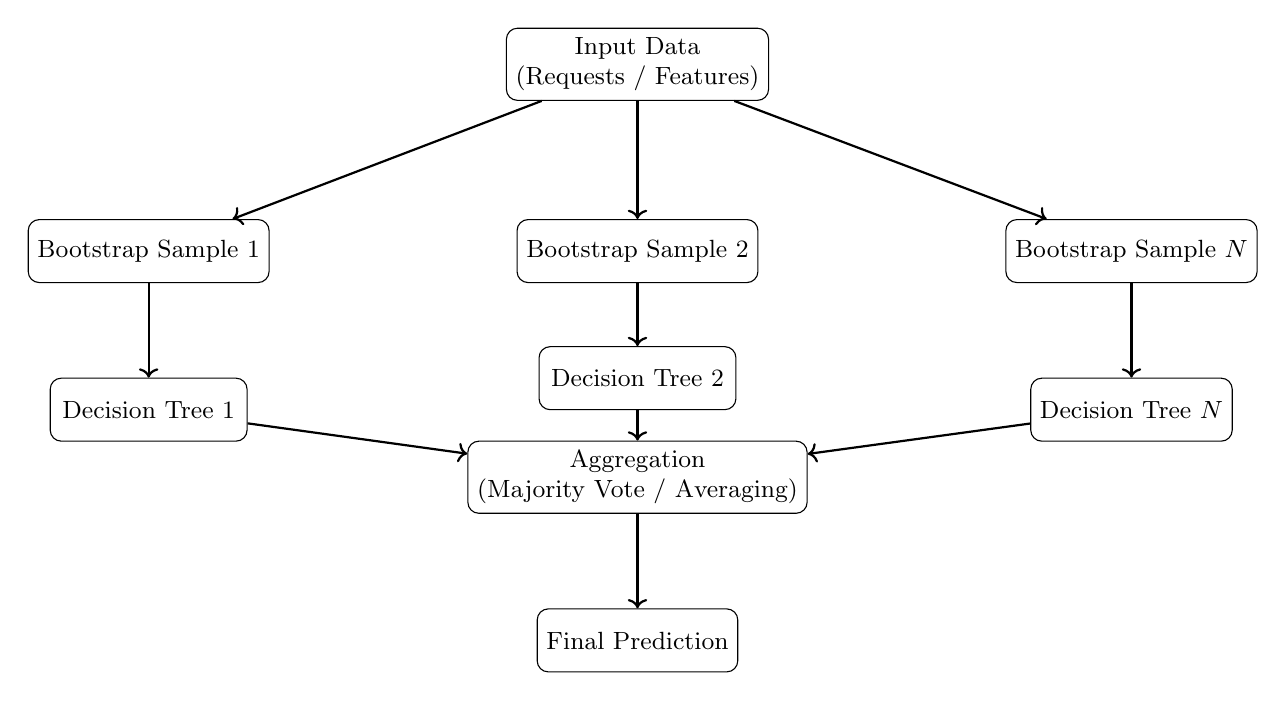
\begin{tikzpicture}[
		font=\small,
		node distance=1.2cm,
		every node/.style={draw, rectangle, rounded corners, align=center, minimum width=2.5cm, minimum height=0.8cm},
		arrow/.style={->, thick}
		]
		
		% Input
		\node (data) {Input Data\\(Requests / Features)};
		
		% Bootstrap samples
		\node (b1) [below left=1.5cm and 3cm of data] {Bootstrap Sample 1};
		\node (b2) [below=1.5cm of data] {Bootstrap Sample 2};
		\node (b3) [below right=1.5cm and 3cm of data] {Bootstrap Sample $N$};
		
		% Trees
		\node (t1) [below=1.2cm of b1] {Decision Tree 1};
		\node (t2) [below=0.8cm of b2] {Decision Tree 2};
		\node (t3) [below=1.2cm of b3] {Decision Tree $N$};
		
		% Aggregation
		\node (agg) [below=2cm of b2, minimum width=4cm] {Aggregation\\(Majority Vote / Averaging)};
		
		% Output
		\node (out) [below=1.2cm of agg] {Final Prediction};
		
		% Arrows
		\draw[arrow] (data) -- (b1);
		\draw[arrow] (data) -- (b2);
		\draw[arrow] (data) -- (b3);
		
		\draw[arrow] (b1) -- (t1);
		\draw[arrow] (b2) -- (t2);
		\draw[arrow] (b3) -- (t3);
		
		\draw[arrow] (t1) -- (agg);
		\draw[arrow] (t2) -- (agg);
		\draw[arrow] (t3) -- (agg);
		
		\draw[arrow] (agg) -- (out);
		
	\end{tikzpicture}
	\caption{Architecture of a Random Forest Classifier}
\end{figure}
Ensemble Learners like Random Forests and XGBoost are widely used for classification tasks. The architecture of Random Forests is visualized as a parallel set of trees, where each tree is a decision tree.
\begin{figure}[h]
	\centering
	\includegraphics[height=6cm]{random-forest}
	\caption{Random Forest Illustration (reproduced from Janosh\cite{riebesell_diagrams_2020})}	
\end{figure}


\newpage
\section{Support Vector Machine}
A Support Vector Machine finds the most optimal \textbf{hyperplane} which acts as the decision boundary between the classes with maximal margin from support vectors. In general, using a \textit{linear kernel function}, if there are ~$p$~ features in the data, the hyperplane is ~$p-1$~ dimensional. 
\begin{figure}[h]
	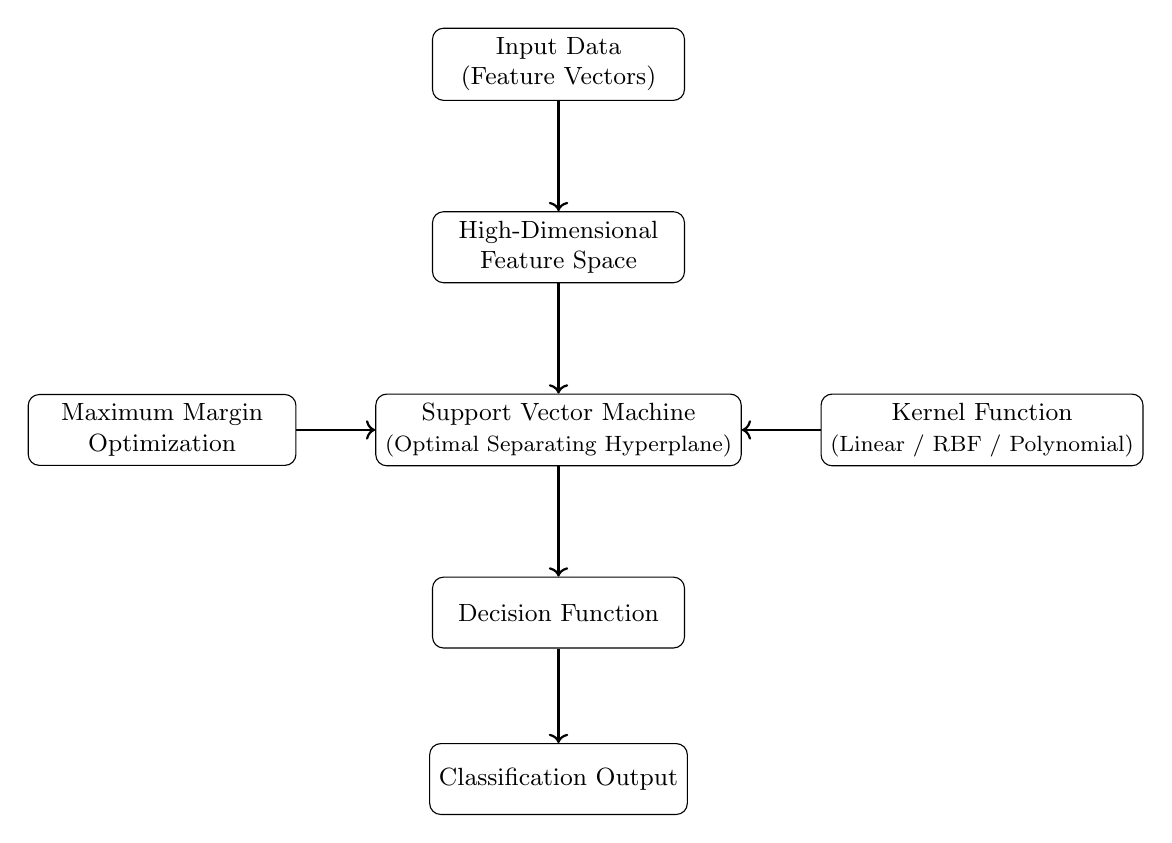
\begin{tikzpicture}[
		font=\small,
		node distance=1.3cm,
		every node/.style={draw, rectangle, rounded corners, align=center, minimum width=3.2cm, minimum height=0.9cm},
		arrow/.style={->, thick}
		]
		
		% Input
		\node (data) {Input Data\\(Feature Vectors)};
		
		% Feature space
		\node (features) [below=1.4cm of data] {High-Dimensional\\Feature Space};
		
		% SVM core
		\node (svm) [below=1.4cm of features, minimum width=4.5cm] 
		{Support Vector Machine\\
			\footnotesize{(Optimal Separating Hyperplane)}};
		
		% Margins
		\node (margin) [left=1cm of svm, minimum width=3.4cm] 
		{Maximum Margin\\Optimization};
		
		% Kernel
		\node (kernel) [right=1cm of svm, minimum width=3.4cm] 
		{Kernel Function\\
			\footnotesize{(Linear / RBF / Polynomial)}};
		
		% Decision
		\node (decision) [below=1.4cm of svm] {Decision Function};
		
		% Output
		\node (out) [below=1.2cm of decision] {Classification Output};
		
		% Arrows
		\draw[arrow] (data) -- (features);
		\draw[arrow] (features) -- (svm);
		\draw[arrow] (svm) -- (decision);
		\draw[arrow] (decision) -- (out);
		
		\draw[arrow] (margin) -- (svm);
		\draw[arrow] (kernel) -- (svm);
		
	\end{tikzpicture}
	\caption{Architecture of a Support Vector Machine (SVM) Classifier}
\end{figure}
\section{TF-IDF}
Term Frequency-Inverse Document Frequency (TF-IDF) is a text mining method that scores word importance in a document relative to a whole collection (corpus), balancing how often a word appears in one text called as Term Frequency (TF) with how rare it is across all texts, called as Inverse Document Frequency (IDF), giving high scores to unique, relevant keywords for tasks like search engines, text classification, and topic modeling.
This vectorization provides vector representation of data with ample features for many natural language processing problems.  

\chapter{Problem Formulation}
Contemporary Web Application Firewall systems are based on rule based sets, which are largely successful but can not protect from patterns not known to them. When a new pattern is found in 0-day, it is not easy to update the rule set. They struggle to detect obfuscated, polymorphic or zero-day injection patterns. 
Recent studies have explored the usage of Machine Learning and Deep Learning for detecting injection attacks which may be employed in an agent driven architecture. Deep Learning outperforms Machine Learning, but the challenge remains of overfitting, data size, robustness to noise and most importantly, performance metrics. Deep Learning models are upto 600 times slower per sample, making them an expensive trade for a high bandwidth application of a reverse proxy server. 
\section{Problem Statement}
To design and implement a Agent Based Web Application Firewall which employs reflex agents powered by Machine Learning Models, namely SVM and XGBoost, to detect and mitigate Injection attacks in real time.
\section{Constraints and Scope}
\begin{enumerate}
	\item The system currently focuses on SQL Injection and XSS only, given their severity and broad access points.
	\item It is trivial to extend from HTTP to HTTPS, so only HTTP 1.1 has been prototyped.
	\item Only XGBoost and SVM models have been implemented, given the research and reasons. 
	\item Encrypted Traffic and other web vulnerabilities remain out of scope for this work.
\end{enumerate}

\chapter{Proposed Work}
In this project, a Web Application Firewall (WAF) is proposed that operates as a reverse proxy between clients and the protected web application. The proposed system employs reflex agents to inspect incoming HTTP requests and take immediate actions based on the inferred threat level.

The architecture consists of modular middleware components, each responsible for detecting a specific class of web attacks. In the current implementation, the system focuses on SQL Injection (SQLi) and Cross-Site Scripting (XSS) attacks. For each incoming request, relevant features are extracted from the request payload and forwarded to machine learning–based detection modules.

To enable efficient and real-time detection, Support Vector Machine (SVM) and XGBoost classifiers are utilized due to their relatively low inference latency and robustness in handling noisy and high-dimensional data. Based on the classification output, the reflex agent takes an appropriate action, such as allowing the request, blocking it, or logging it for further analysis.

The proposed WAF is designed to be lightweight, extensible, and scalable, allowing additional detection agents or models to be integrated in the future. By combining machine learning–based detection with an agent-oriented decision mechanism, the system aims to improve adaptability against evolving attack patterns while maintaining performance suitable for real-time web traffic inspection.

The WAF is tested with DVWA (Damn Vulnerable Web Application) which poses as a suitable vulnerable application for safe and practical demonstration purposes.

\chapter{System Design}
\begin{figure}[h]
	\centering
	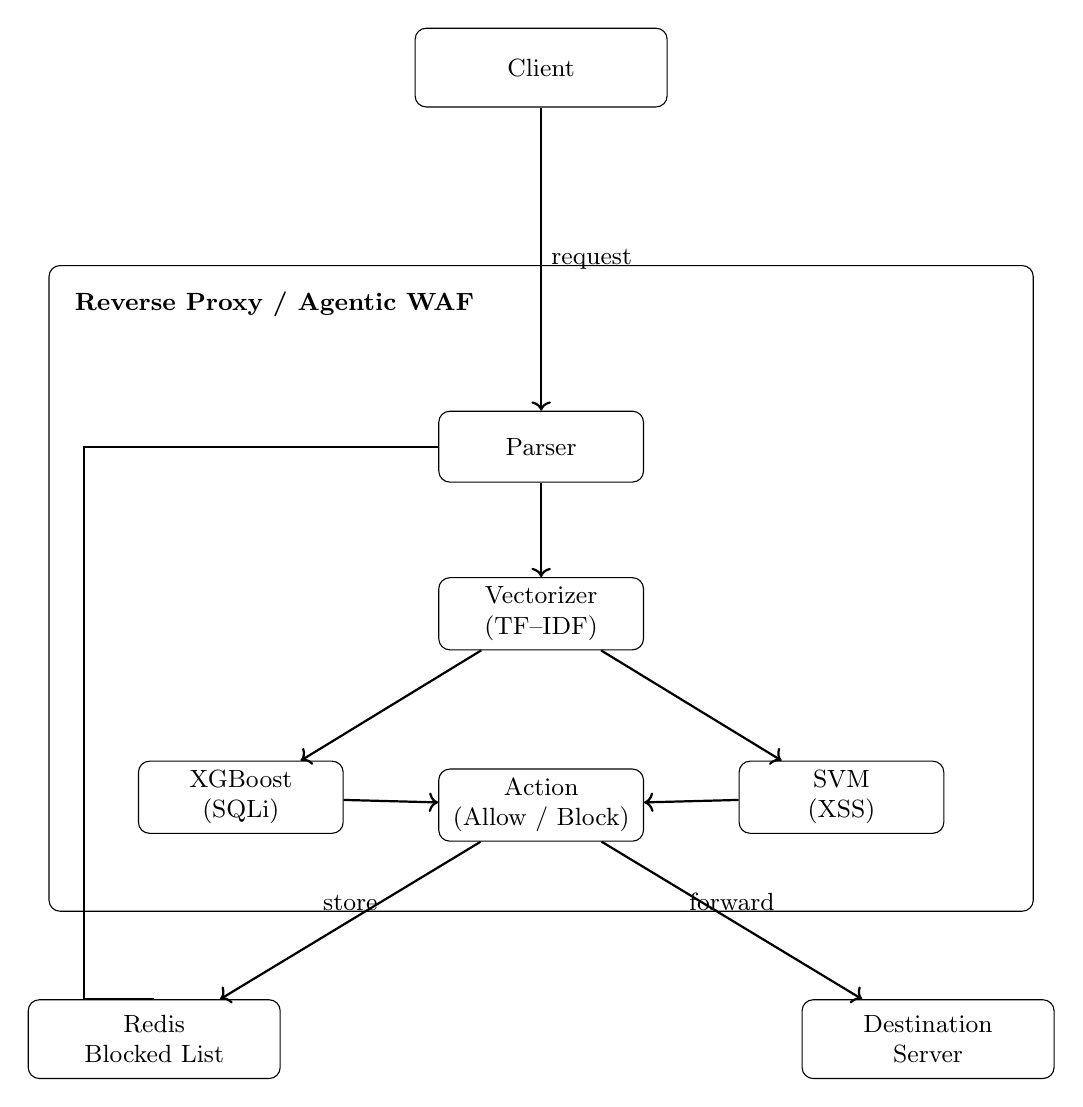
\begin{tikzpicture}[
		font=\small,
		node distance=1.5cm,
		box/.style={
			draw,
			rectangle,
			rounded corners,
			align=center,
			minimum width=3.2cm,
			minimum height=1cm
		},
		smallbox/.style={
			draw,
			rectangle,
			rounded corners,
			align=center,
			minimum width=2.6cm,
			minimum height=0.9cm
		},
		arrow/.style={->, thick}
		]
		
		% ---- Client ----
		\node[box] (client) {Client};
		
		% ---- Proxy / Agentic WAF Container ----
		\node[box, below=2cm of client, minimum width=12.5cm, minimum height=8.2cm] (waf) {};
		
		\node[anchor=north west] at ([xshift=6pt,yshift=-6pt]waf.north west)
		{\textbf{Reverse Proxy / Agentic WAF}};
		
		% ---- Inside WAF ----
		\node[smallbox] (parser) at ([yshift=1.8cm]waf.center) {Parser};
		
		\node[smallbox, below=1.2cm of parser] (vectorizer) {Vectorizer\\(TF--IDF)};
		
		\node[smallbox, below left=1.4cm and 1.2cm of vectorizer] (rf)
		{XGBoost\\(SQLi)};
		
		\node[smallbox, below right=1.4cm and 1.2cm of vectorizer] (svm)
		{SVM\\(XSS)};
		
		\node[smallbox, below=1.5cm of vectorizer] (action)
		{Action\\(Allow / Block)};
		
		% ---- External Systems ----
		\node[box, below left=2cm and 2cm of action] (redis)
		{Redis\\Blocked List};
		
		\node[box, below right=2cm and 2cm of action] (server)
		{Destination\\Server};
		
		% ---- Arrows ----
		\draw[arrow] (client) -- node[right]{request} (parser);
		\draw[arrow] (parser) -- (vectorizer);
		
		\draw[arrow] (vectorizer) -- (rf);
		\draw[arrow] (vectorizer) -- (svm);
		
		\draw[arrow] (rf) -- (action);
		\draw[arrow] (svm) -- (action);
		
		\draw[arrow] (action) -- node[above]{store} (redis);
		\draw[arrow] (action) -- node[above]{forward} (server);
		\coordinate (bend) at ($(parser.west)+(-4.5,0)$);
		
		\draw[thick] (parser.west) -- (bend) |- (redis.north);
		
		
	\end{tikzpicture}
	\caption{Architecture of Agentic Web Application Firewall using Reflex Agents}
\end{figure}
\section{Client}
The client sends HTTP requests to the reverse proxy server. It is assumed that it may act as a threat actor.  
\section{Destination Server} 
This is the server hosting the vulnerable application. For demonstration purposes, this application is chosen to be DVWA (Damn Vulnerable Web Application)
\section{Reverse Proxy} 
The Reverse Proxy Server will analyze the request before forwarding it to the vulnerable application server.
\subsection{Parser}
Parses incoming HTTP requests for their headers, meta data and form data. It also presents the request IP to the in-memory database to check if the user is already blocked. 
\subsection{Vectorizer}
The TF-IDF Vectorizer is a part of the ML Pipeline that vectorizes the request inputs for Classification.
\subsection{XGBoost}
This classifies the user input against SQL Injection. 
\subsection{SVM}
This classifies the user input against XSS.
\subsection{Action}
This automaton (program) performs an AND operation to decide whether the input is safe. 
\section{Redis}
Redis acts as a in-memory database for WAF settings and blocked IPs. The blocked IPs are stored in form of \textbf{Tries} for ~$O(1)$~ time access as IPV4 addresses are essentially 4 octets. Redis also ensures scalability and consistency of the server.

\chapter{Implementation}
\section{Technology Stack}
\begin{itemize}
	\item Server Language: Python 3
	\item Framework: aiohttp - Asynchronous IO HTTP Server
	\item Vectorizer: TfidfVectorizer (sklearn)
	\item Machine Learning: scikit-learn
	\item Database: Redis
	\item Desktop Application: Tkinter
	\item SIEM: HTML, CSS, Tailwind, Javascript
	\item Deployment: Docker 
\end{itemize}

\section{Reverse Proxy Implementation}
The reverse proxy is implemented using the aiohttp asynchronous framework. It listens for incoming HTTP requests and forwards them to the upstream server after inspection. All HTTP methods, headers, query parameters, and request bodies are preserved during forwarding, except Hop-by-hop headers that are meant to change with each node in the network path for consistency. 

\section{Parser}
The request parser extracts relevant components such as URL path, query parameters, headers, and request body. Inputs are normalized to a standard textual format before feature extraction.

\section{Vectorizer}
Feature extraction is performed using TF–IDF vectorization. Parsed request data is transformed into numerical feature vectors compatible with machine learning classifiers.

\section{Machine Learning}
\subsection{SVM - XSS}
SVM is trained with linear kernel on an open dataset from Kaggle by Hussain (2020)\cite{xss_dataset_hussain_2020}. Data has been synthetically augmented to balance with natural queries using Claude, as the dataset was meant for classification of SQLi detection within SQL Queries only. 

\subsection{XGBoost - SQL Injection}
XGBoost is trained on an open dataset from GitHub by Kumar(2024)\cite{sqlqueriesdata_ankitkumar_2024}. Data has been synthetically augmented to balance with natural queries using Python's \textbf{Faker} library. \\
Tree parameters: max\_depth is set to 4, min\_child\_weight to 10, gamma=2, reg\_alpha=1 and reg\_lambda=3
\subsection{Miscellaneous}
Redis and DVWA are setup with Docker. Launch window is made with Tkinter. SIEM is made with HTML CSS and Javascript. 

\chapter{Result Analysis}
A fully working model has been constructed, with the XGBoost's efficiency 98.54\% and SVM's efficiency 96.15\%. Appropriate Demonstrations with DVWA provided.   

\begin{table}[h]
	\centering
	\caption{Performance Evaluation of Machine Learning Models}
	\label{tab:results}
	\begin{tabular}{|l|l|c|c|c|c|}
		\hline
		\textbf{Model} & \textbf{Attack Type} & \textbf{Accuracy} & \textbf{Precision} & \textbf{Recall} & \textbf{F1-score} \\
		\hline
		XGBoost & SQL Injection & 98.54\% & 0.96 & 0.98 & 0.97 \\
		\hline
		SVM & XSS & 96.15\% & 0.94 & 0.95 & 0.95 \\
		\hline
	\end{tabular}
\end{table}

The server works with adding minimal latency.

\chapter{Conclusion, Limitations and Future Scope}
\section{Conclusion}
This project presented an Agentic Web Application Firewall implemented using a reverse-proxy architecture with reflex agents. The system intercepts incoming client requests, performs feature extraction, and applies machine learning models to detect SQL injection and cross-site scripting attacks.

Support Vector Machine and XGBoost classifiers were trained and integrated for XSS and SQL injection detection respectively. Experimental results demonstrate that the proposed system is capable of accurately identifying malicious requests while maintaining acceptable inference latency for real-time deployment.

The modular design of the system allows independent improvement of individual components, making it adaptable to evolving web security threats.
\section{Limitations}
Despite its effectiveness, the proposed system has certain limitations. The current implementation focuses only on SQL injection and cross-site scripting attacks and does not address other web vulnerabilities such as CSRF, command injection, or authentication bypass attacks.

The machine learning models are trained on specific datasets, which limits generalization to highly novel or adversarial payloads, which would require a training feedback loop. The system also returns false positives at inputs crafted to resemble SQL Injection or XSS payloads. Additionally, the system currently performs request-level analysis and does not incorporate long-term user behavior profiling or session-based anomaly detection with unsupervised learning. 

Scalability may also be impacted as the number of deployed models increases, potentially affecting inference latency under very high traffic conditions.
\section{Future Scope}
The proposed system can be extended in several directions. The covered vulnerability classifiers can be improved by combining multiple models, or using Deep Learning for stricter security policies in a federated manner. Additional detection modules can be incorporated to handle a wider range of web vulnerabilities beyond SQL injection and XSS. 

Future work may include integrating user behavior analysis and clustering techniques to enable adaptive and context-aware security policies. The use of lightweight deep learning models or ensemble decision strategies can also be explored to improve detection accuracy while maintaining low latency.



\bibliographystyle{IEEEtran}
\bibliography{references}


\end{document}